\section{Signal analysé en posturographie statique}

\subsection{Pression plantaire}

Les pressions plantaires mesurent la répartition des forces sous les pieds au niveau des zones d’appui.
Ces pressions sont capturées par des capteurs disposés sur une surface ou intégrées dans des semelles.
Ces mesures permettent d’identifier les points de pression maximale et minimale, fournissant des données sur la statique et la dynamique du pied.
Les centres de pression sont calculés à partir des variations de pression.
Ils reflètent les ajustements dynamiques de la posture en réponse aux déséquilibres.
Les mesures de ces signaux nous permettent de cartographier les zones d'appui et de visualiser les charges appliquées sur les pieds.
On peut alors identifier les zones à risque de pathologie (comme l’hallux valgus ou la fasciite plantaire).
L'évaluation des déséquilibres ou anomalies dans la distribution des forces est alors possible.
Les études sont appliquées en podologie et orthopédie, pour détecter les troubles plantaires ou les anomalies posturales.
Elles sont aussi utilisées pour suivre les progrès post-blessures ou post-chirurgie de patients.
Enfin, on peut aussi les mener dans le but d’optimiser les performances athlétiques en analysant les impacts au sol.

\subsection{Méthode d'enregistrement}

Les plateformes stabilométriques mettent l’accent sur l'étude des mouvements posturaux en évaluant les forces verticales et les déplacements dans les plans horizontal et vertical.
Ces plateformes disposent fréquemment d’instruments additionnels, comme des surfaces instables ou des systèmes de visualisation interactifs pour perturber l'équilibre et examiner les réactions compensatoires du patient.
Ces dispositifs sont utilisés pour évaluer la stabilité posturale en position debout, notamment chez des patients atteints de troubles neurologiques ou vestibulaires.
Ils sont également utilisés pour détecter les déficiences proprioceptives et pour la rééducation.
En gériatrie, ils permettent d'évaluer les risques de chute, et en sport, ils servent à optimiser les stratégies d' équilibre.

\textbf{Exemples :}
\begin{itemize}
  \item Stabilo Stabilometric Platform
  \item Plateforme Satel
\end{itemize}

\begin{figure}[ht]
  \centering
  \begin{subfigure}[b]{0.45\textwidth}
    \centering
    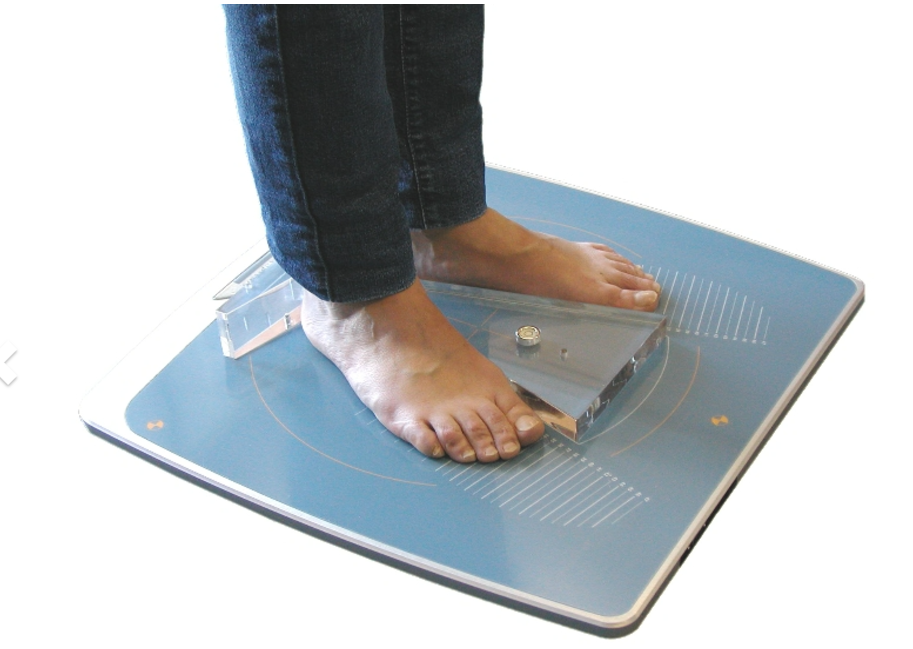
\includegraphics[height=5cm]{images/pression_plantaire/plateforme-stabilometrique.png}
    \caption{Plateforme stabilométrique}\label{fig:plateforme_stabilometrique}
  \end{subfigure}
  \begin{subfigure}[b]{0.45\textwidth}
    \centering
    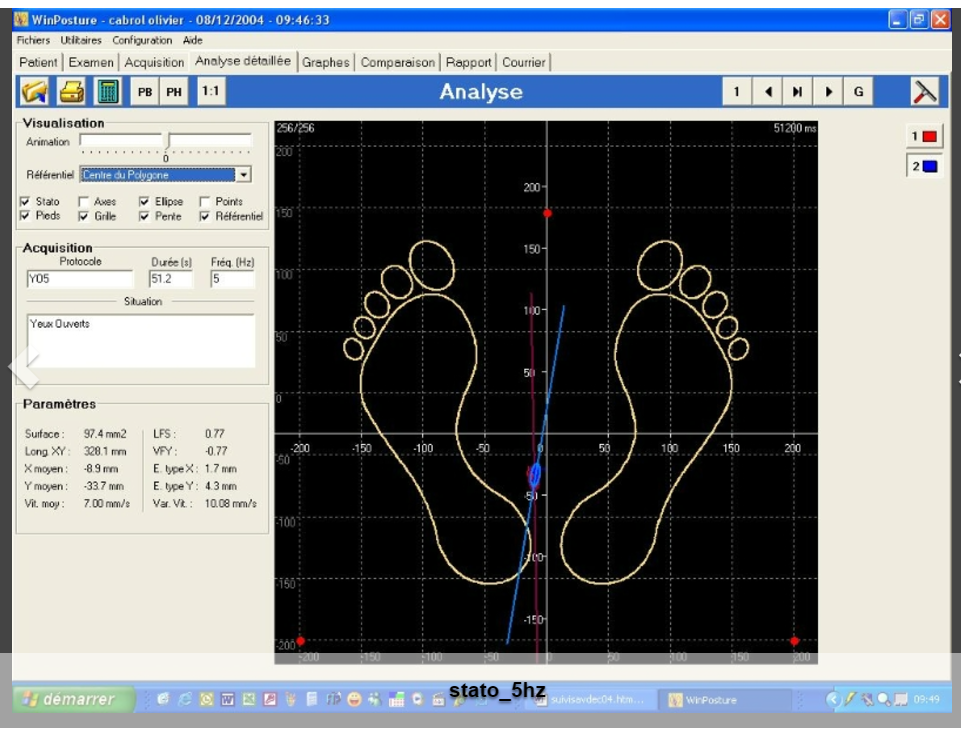
\includegraphics[height=5cm]{images/pression_plantaire/winposture.png}
    \caption{Logiciel Winposture}\label{fig:winposture}
  \end{subfigure}
  \begin{subfigure}[b]{0.45\textwidth}
    \centering
    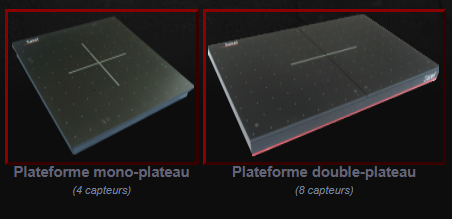
\includegraphics[height=5cm]{images/pression_plantaire/satel.png}
    \caption{Plateforme stabilométrique Satel}\label{fig:satel}
  \end{subfigure}
  % \caption{Ill}\label{fig:exemple_plateforme_force}
\end{figure}

\begin{figure}[ht]
  \centering
  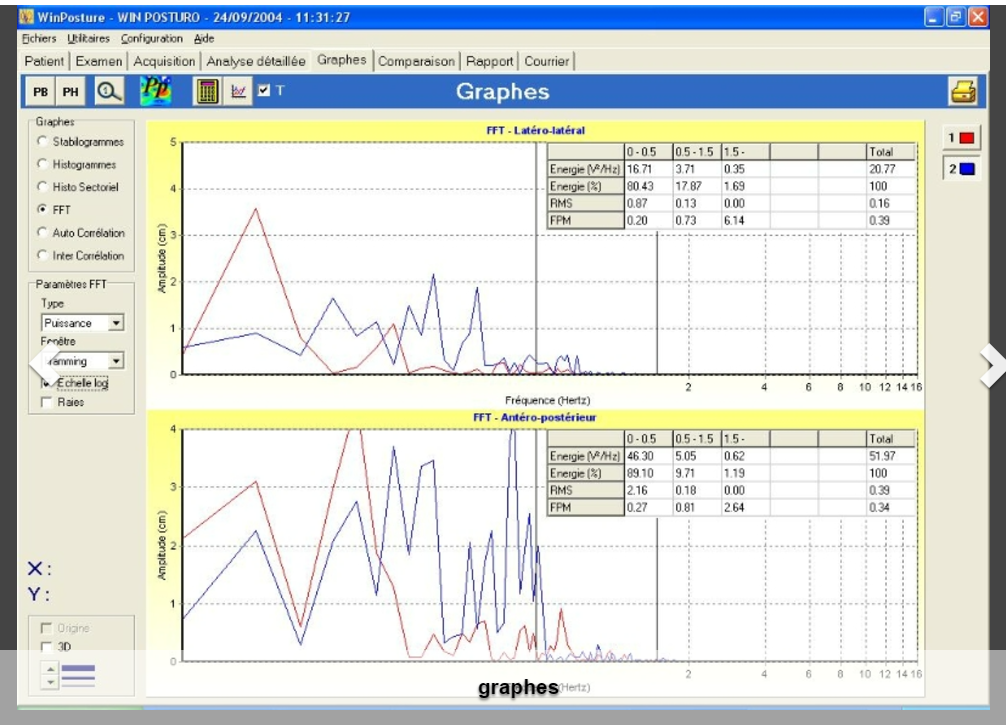
\includegraphics[height=10cm]{images/pression_plantaire/winposture2.png}
  \caption{Logiciel Winposture}\label{fig:winposture2}
\end{figure}
